\section{Network Layer Attacks}

\subsection{IP Spoofing}
An attacker host can try to impersonate another host by spoofing the IP address of that host in its IP datagrams. IP spoofing is used to:

- impersonate sources of security-critical information (e.g., DNS servers) 

- exploit address-based authentication in higher-level protocols 

- evade attack detection based on IP address 

One type of IP spoofing is called blind IP spoofing, where an attacker sends IP packets that forge the source IP address of another host, and the receiver will send a reply back to the forged address. However, the attacker usually does not have access to the reply. 

On the Internet, on-path attackers can see the traffic, making spoofing easy. However, for off-path attackers, since they cannot see the traffic, they have to spoof blindly. They often need to guess header values to succeed, or rely on brute force. An attacker can spoof if they have a reasonable chance of success. 

\subsection{Autonomous System}
A large collection of networks under one organization is called an Autonomous System (AS), where an AS manages its own internal routing. ASes are interconnected to form the Internet, which can be considered a network of networks. Each AS determines which neighboring AS to send a packet to, and this inter-network routing is specified by the \textbf{Border Gateway Protocol (BGP)}.

Consider a device sending an IP datagram to the gateway. If the destination is within the same AS, routers inside the AS will perform internal routing. Otherwise, the packet is forwarded to another AS. Between different ASes (inter-network routing), routing decisions are specified by \textbf{BGP}. 

In an edge AS, where users connect directly, mechanisms such as ingress filtering can be applied to restrict IP spoofing (i.e., blocking packets with forged source IP addresses). However, since deployment is not universal and attackers can forge source addresses, only a fraction of edge ASes enforce such filtering. This enables various attacks based on IP spoofing, including blind spoofing. 

\subsection{Routing}
The host uses a routing table to maintain information about how to reach a destination IP address. Routing is performed through the following steps:

- search for a matched host in the table 

- search for a matched network in the table 

- search for a default entry 

- an error \texttt{Host/network unreachable} is returned if no match is found 

Routing tables can be set statically at system startup time or dynamically using routing protocols. 

\subsection{Internet Control Message Protocol (ICMP)}
Internet Control Message Protocol (ICMP) is used to exchange control or error messages about the delivery of IP datagrams. The messages are encapsulated inside IP datagrams, and they can be:

- requests 

- responses 

- errors (including the header and a portion of the payload of the offending IP datagram) 

ICMP Echo messages are used by the ping program to test connectivity. However, ICMP Echo Request messages can also be used to map the hosts of a network. This can be done by sending ICMP echo datagrams to all hosts in a subnet, then collecting the replies and determining which hosts are alive. This can also be used to perform Denial of Service (DoS) attacks. 

ICMP messages are also used by gateways to indicate that a datagram cannot be delivered, such as:

- Network unreachable 

- Host unreachable 

- Protocol unreachable 

- Port unreachable 

- Fragmentation needed but “don’t fragment” flag set 

- Destination host unknown 

- Destination network unknown 

In addition, forged destination unreachable messages can cut off hosts from the network, which is also a form of DoS attack.

\section{Transport Layer Attacks}

\subsection{User Datagram Protocol (UDP)}
The User Datagram Protocol is a transport layer protocol. It provides a connectionless, unreliable, and best-effort datagram delivery service. Similar to IP, delivery, integrity, ordering, non-duplication, and bandwidth are all not guaranteed. 

This protocol introduces the port abstraction, allowing one to communicate with different components on the same IP address, and it is often used for multimedia applications and for services based on a request-reply scheme (e.g., DNS). 

\begin{figure}[H]
  \centering
  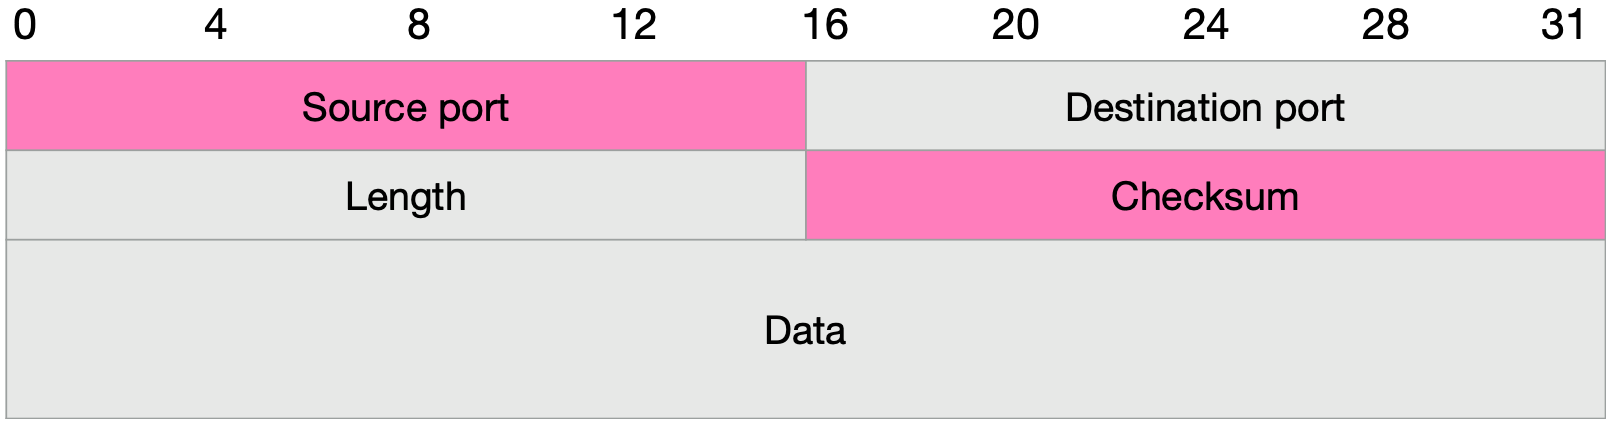
\includegraphics[width=0.7\textwidth]{Figure/UDP.png}
  \caption{UDP Packet}
\end{figure}

\begin{remark}
  The source port and checksum are optional in IPv4. 
\end{remark}

For UDP attacks, there are:

- UDP spoofing: similar to IP spoofing  

- UDP hijacking: a variation of UDP spoofing attacks  

- UDP port scan  

This is used to determine which UDP services are available. A zero-length UDP packet is sent to each port, and an ICMP ``port unreachable'' error message indicates that certain ports are unavailable. However, the scan rate can be limited by the TCP/IP stack implementation. 

- DoS  

UDP does not have a session concept, so it can be used as a basis for DoS attacks. The receiver cannot meaningfully block UDP packets in most cases, i.e., it is difficult to effectively distinguish between legitimate and attack traffic. 

\subsection{Transmission Control Protocol (TCP)}
Transmission Control Protocol is another transport layer protocol. It provides a connection-oriented, reliable stream delivery service, i.e., delivery, ordering, and non-duplication are all guaranteed. 

TCP allows two hosts to establish a virtual circuit (connection), identified by the IP address and port of the source and the destination. The virtual circuit consists of two streams (full-duplex connection). The IP address and port tuple is sometimes called a socket, and the two endpoints form a socket pair, which defines one TCP connection. 

\begin{figure}[H]
  \centering
  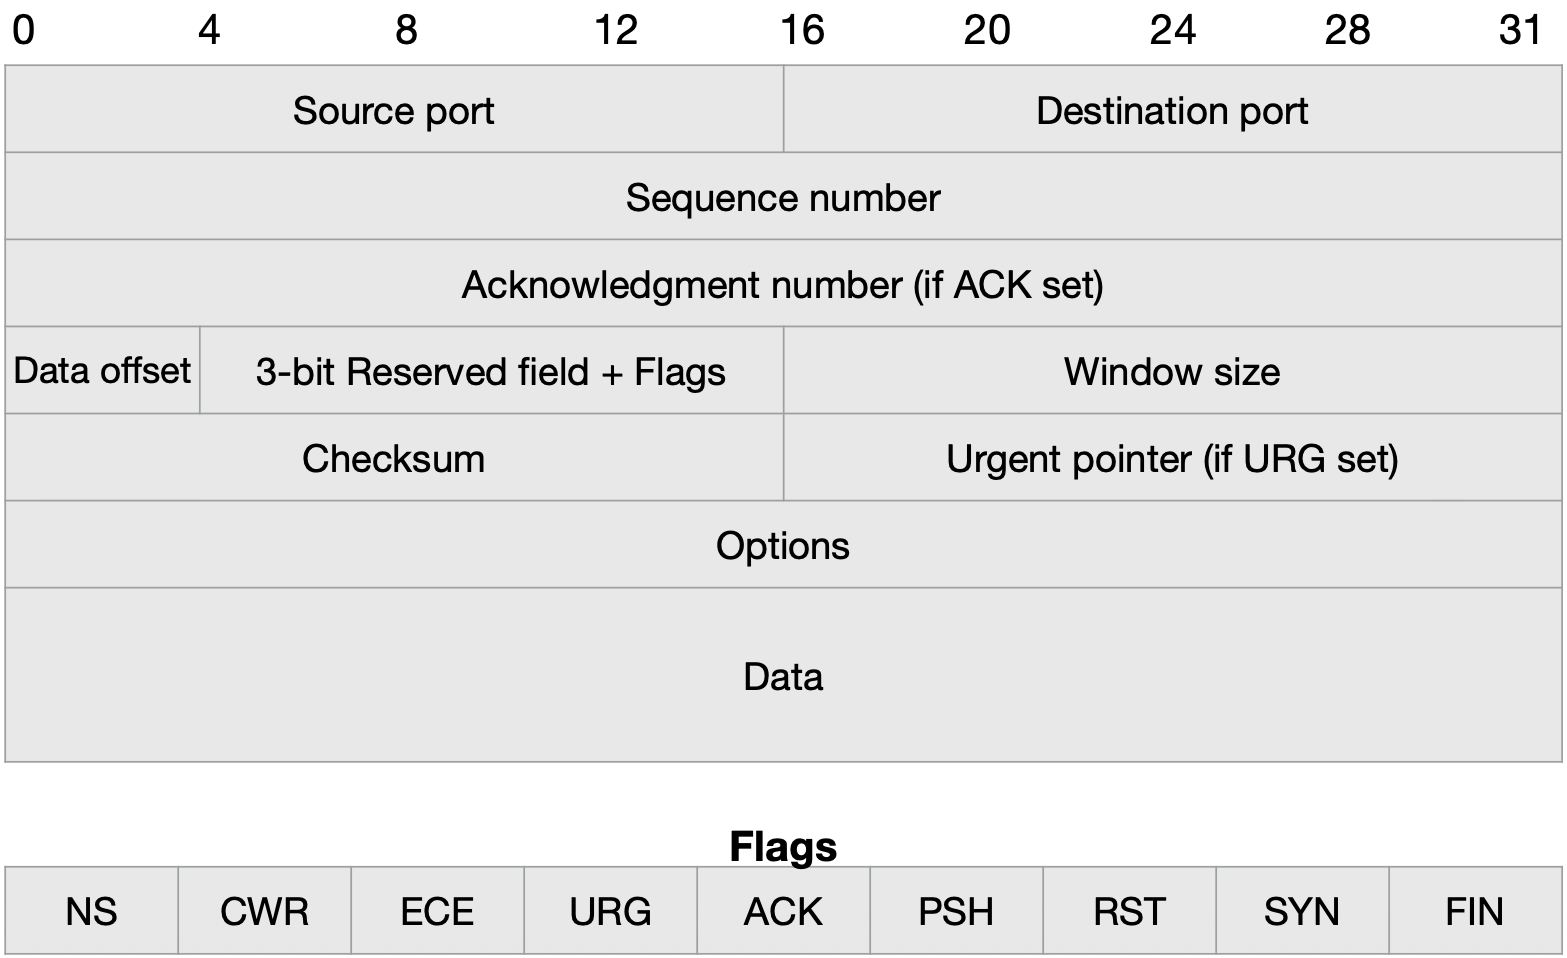
\includegraphics[width=0.7\textwidth]{Figure/TCP.png}
  \caption{TCP Packet}
\end{figure}

Like UDP, TCP ports are associated with OS processes. TCP uses sequence and acknowledgment numbers to manage retransmission, duplication, and flow control. The sequence number represents the relative position of the TCP segment in the stream, while the acknowledgment number specifies the position of the next byte expected from the stream. 

\subsubsection{TCP Flags}
Flags in TCP are used to manage a connection:

- SYN: start connection  

Requests synchronization of sequence/acknowledgment numbers (set in connection setup packets).  

- ACK: acknowledge data  

Indicates that the acknowledgment number is valid (set in all packets except the first one).  

- FIN: finish sending  

Requests to terminate one stream (last packet from the sender).  

- RST: reset connection  

Requests to immediately reset the connection.  

- URG: urgent data  

Indicates that the Urgent Pointer is valid.  

- PSH: deliver immediately  

Requests to push buffered data to the receiving application.  

\subsubsection{TCP Window}
The TCP window is used to perform flow control. A segment is accepted only if its sequence number is inside the window starting from the current ACK number, i.e., 
\[
  \text{ACK number} \leq \text{sequence number} \leq \text{ACK number} + \text{Window} 
\]

The window size can be dynamically changed to adjust the amount of data sent by the sender. 

\subsubsection{TCP Connection}
To set up a connection, the server listens on a specific port, and the client requests to establish a connection to the port by sending a SYN request with an initial sequence number \texttt{Sc}. The server then accepts the connection by replying with a SYN/ACK packet. The server sets an initial sequence number \texttt{Ss}, and the acknowledgment number is \texttt{Sc + 1}. The client then acknowledges to complete the setup, where the sequence number becomes \texttt{Sc + 1} and the acknowledgment number becomes \texttt{Ss + 1}.  

To shut down a connection, one end (A) sends a FIN packet to indicate the shutdown of half of the connection. The other end (B) replies with an ACK packet. A will still reply with ACK packets if B continues sending packets in the other stream. To close the other stream, B also sends a FIN packet, and A replies with an ACK packet.  

\subsubsection{TCP Port Scan}
One threat to TCP is port scanning. This is used to determine which TCP services are available.  

\textbf{Normal scanning}  

The scanner tries to establish a TCP connection with an arbitrary port. The port is available if the connection is successful, which creates many logs and connections.  

\textbf{SYN scanning}  

After the scanner sends a SYN request, the port is available if the server returns a SYN/ACK; otherwise, an RST packet is usually returned. The scanner then sends an RST packet to terminate the ``connection'' if a SYN/ACK is returned. This connection is never fully established, and the event may not be logged by the operating system or application.  

\textbf{FIN scanning}  

The port is open if the FIN packet is ignored, and closed if the server sends an RST packet. In Windows systems, an RST is sent back in any case. There are also variations of this scanning technique, such as:

- Xmas: FIN, PSH, and URG set  

- Null: no flags set  

\subsubsection{Disruption}
Normally, a TCP connection is terminated by each end of the connection by sending a FIN packet, and the other end must reply with an ACK packet.  

However, one can abruptly terminate the connection by sending an RST packet. This is unilateral; no ACK is expected or needed, and it is only accepted by the peer if the packet has the correct sequence number. This is called RST injection.  

In RST injection, an attacker can disrupt a TCP connection if they know the port and sequence number.  

\subsubsection{Data Injection}
An attacker can inject data into a TCP stream if they know the port and sequence number. This is also known as TCP connection hijacking. It is also possible for an off-path attacker to inject data into a TCP connection as long as they can guess or infer the correct sequence number and port.  

\subsubsection{TCP Spoofing}
TCP disruption and data injection both require that the attacker can spoof the IP address of a sender and knows the sequence number and port number. This can be easily done by a MITM attacker.  

For TCP blind spoofing, it is much more difficult but still possible. For example, A sends a TCP SYN segment that spoofs the IP address of C with \texttt{Sc} as the sequence number to S. Then S replies with a SYN/ACK segment to C with \texttt{Ss} as the sequence number. The segment is ignored by C, and A does not receive the reply from S.  

Therefore, A must send an ACK segment to S to finish the connection setup with \texttt{Ss + 1} as the ACK number. A has to respond quickly before C sends an RST packet. A may try to infer or guess the sequence number by establishing a real connection with S to predict the sequence number.  

To defend against this, random initial sequence numbers should be used, although implementations may not be perfectly random.  

\subsubsection{TCP SYN Flooding}
An attacker can flood a victim host with many TCP SYN packets. Each SYN packet creates a half-open connection, and the victim host must allocate resources for these incoming connections. This can lead to Denial of Service (DoS).